\begin{figure*}[hbtp]
  \centering
  \subfigure[Runtime in seconds (logarithmic scale) with \textit{GVE-Louvain} and \textit{GVE-Leiden}]{
    \label{fig:gve-compare--runtime}
    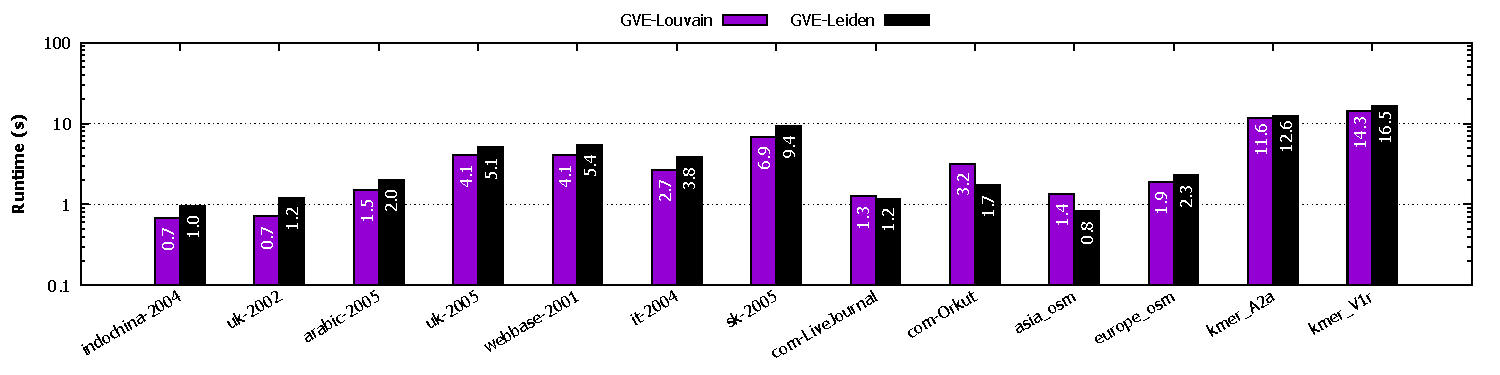
\includegraphics[width=0.98\linewidth]{out/gve-runtime.pdf}
  } \\[-0ex]
  \subfigure[Speedup of \textit{GVE-Leiden} with respect to \textit{GVE-Louvain}. \textit{GVE-Leiden} is generally slower (speedup < $1$) because of additional refinement phase.]{
    \label{fig:gve-compare--speedup}
    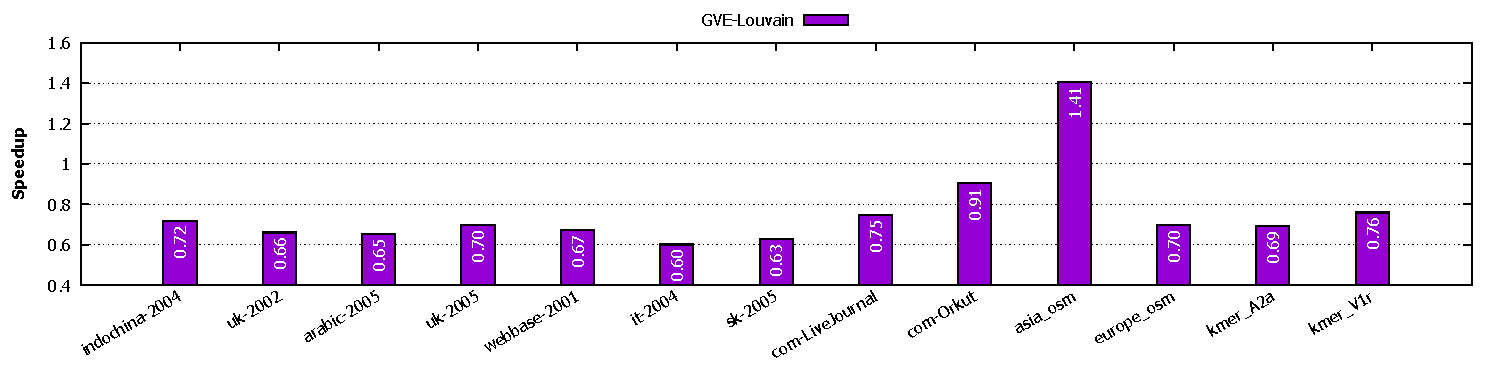
\includegraphics[width=0.98\linewidth]{out/gve-speedup.pdf}
  } \\[-0ex]
  \subfigure[Modularity of communities obtained with \textit{GVE-Louvain} and \textit{GVE-Leiden}.]{
    \label{fig:gve-compare--modularity}
    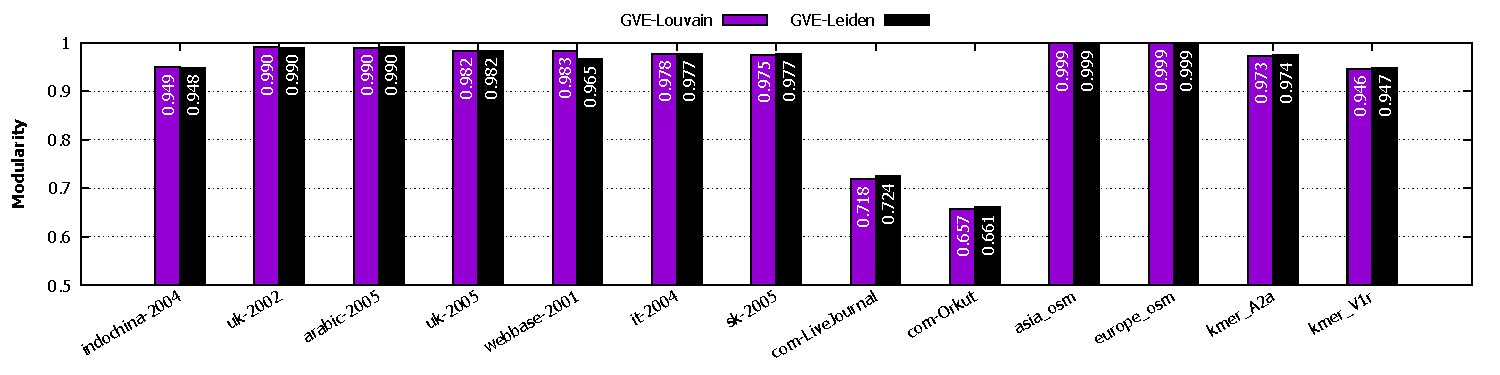
\includegraphics[width=0.98\linewidth]{out/gve-modularity.pdf}
  } \\[-0ex]
  \subfigure[Fraction of disconnected communities (logarithmic scale) with \textit{GVE-Louvain} and \textit{GVE-Leiden}.]{
    \label{fig:gve-compare--disconnected}
    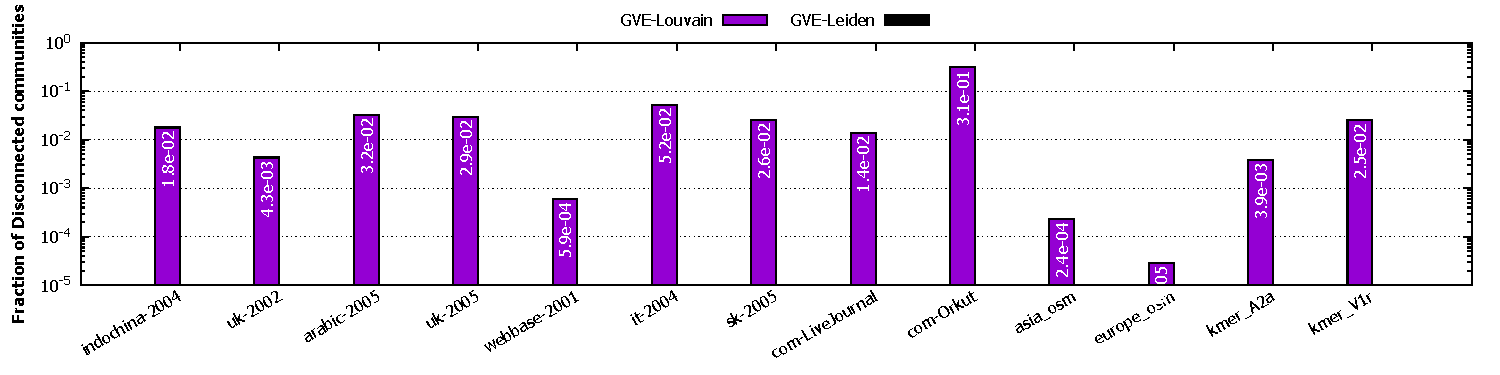
\includegraphics[width=0.98\linewidth]{out/gve-disconnected.pdf}
  } \\[-2ex]
  \caption{Runtime in seconds (log-scale), speedup, modularity, and fraction of disconnected communities (log-scale) with \textit{GVE-Louvain} and \textit{GVE-Leiden} for each graph in the dataset.}
  \label{fig:gve-compare}
\end{figure*}
